\documentclass[12pt]{article}

\usepackage[spanish]{babel}

\selectlanguage{spanish}

\usepackage[utf8]{inputenc}

\usepackage{graphicx}

\title{Iniciando con Fortran}

\author{Jesús Valenzuela Nieblas}

\date{}

\begin{document}

\maketitle

\section{Introducción}

En esta actividad, comenzamos a utilizar Fortran para la creación de pequeños programas que resuelvan ciertos problemas matemáticos

\section{Programas en fortran}

\subsection{Área del círculo}

Se nos pide crear un programa que calcule el área del círculo ingresando como dato únicamente el valor del radio.

\begin{figure}[h]

\centering

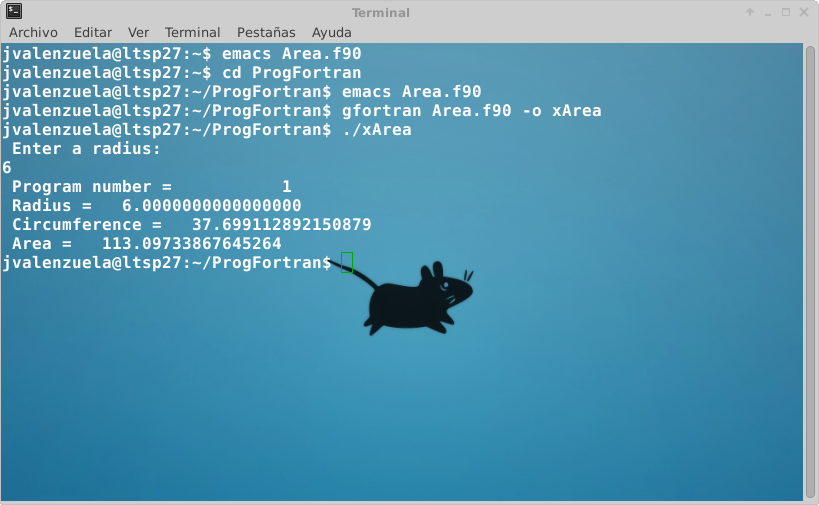
\includegraphics[scale=0.5]{Area.png}

\end{figure}

\begin{verbatim}
! Area . f90 : Calculates the area of a circle, sample program
 Program areacirculo ! Begin main program
  Implicit None ! Declare all variables
   Real *8 :: radius , circum , area ! Declare Reals
   Real *8 :: PI = 4.0 * atan(1.0) ! Declare , assign Real
  Integer :: model_n = 1 ! Declare , assign Ints
   print * , 'Enter a radius:' ! Talk to user
   read * , radius ! Read into radius
  circum = 2.00 * PI * radius ! Calc circumference
  area = radius * radius * PI ! Calc area
  print * , 'Program number =' , model_n ! Print program number
  print * , 'Radius =' , radius ! Print radius
  print * , 'Circumference =' , circum ! Print circumference
  print * , 'Area =' , area ! Print area
 End Program areacirculo ! End main program code

\end{verbatim}

\subsection{Volumen de la esfera}

En esta ocación, se modificó el programa anterior para que calcul el volumen de una esfera ingresando únicamente su radio.

\begin{figure}[h]

\centering

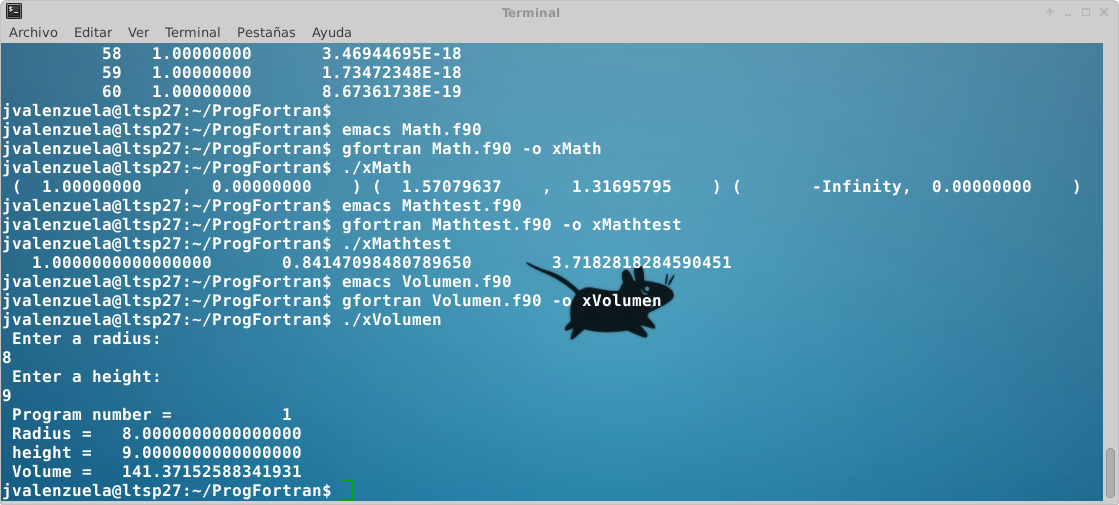
\includegraphics[scale=0.5]{Volumen.png}

\end{figure}

\begin{verbatim}
! Volumen . f90 : Calculates the area of a circle, sample program
 Program volumen ! Begin main program
  Implicit None ! Declare all variables
   Real *8 :: radius , height , volume , newradius ! Declare Reals
   Real *8 :: PI = 4.0 * atan(1.0) ! Declare , assign Real
  Integer :: model_n = 1 ! Declare , assign Ints
   print * , 'Enter a radius:' ! Talk to user
   read * , radius ! Read into radius
   print * , 'Enter a height:' ! Talk to user
   read * , height ! Pide la altura
   newradius = 3 * radius - height
   volume = 0.333333 * PI * height * newradius 
  print * , 'Program number =' , model_n ! Print program number
  print * , 'Radius =' , radius ! Print radius
  print * , 'height =' , height 
  print * , 'Volume =' , volume ! Print area
 End Program volumen ! End main program code
\end{verbatim}

\subsection{Presición de la maquina}

Se pide modificar el código dado para crear un prorama que mida la precisión de la maquina.

\begin{figure}[h]

\centering

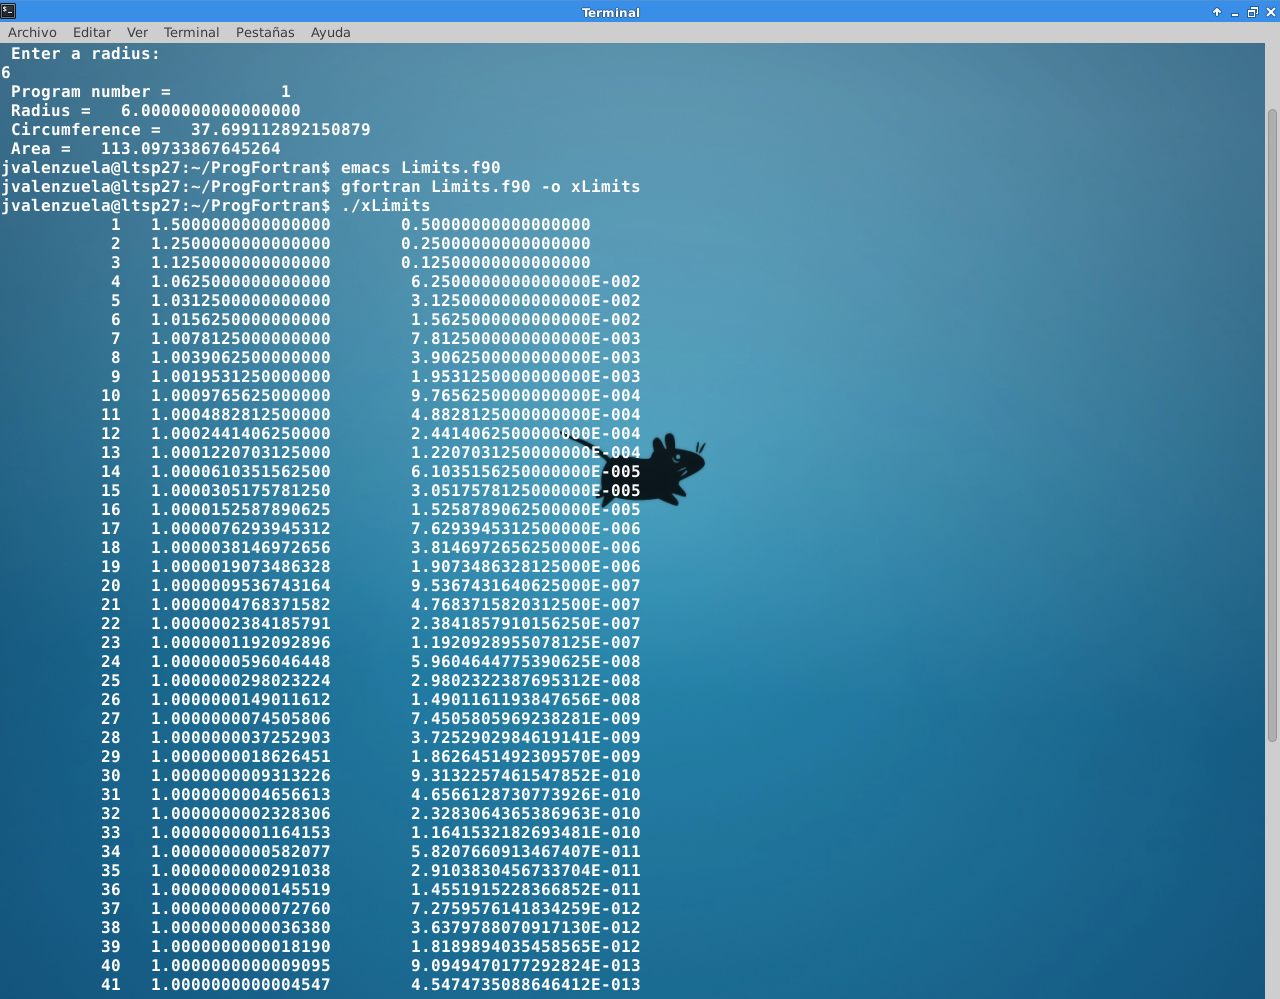
\includegraphics[scale=0.5]{Limits.png}

\end{figure}

\begin{verbatim}
!Limits.f90 Determines machine precision
Program Limits
  Implicit None
  Integer :: i , n
  Real *8 :: epsilon_m , one
  n=60 ! Establece el número de iteaciones
  ! Set initial values:
  epsilon_m = 1.0
  one = 1.0
  ! Within a DO-LOOP, calculate each step and print .
  ! This loop will execute 60 times in a row as i is
  ! incremented from 1 to n (since n = 60) :
  do i =  1, n , 1 ! Begin the do-loop
     epsilon_m = epsilon_m / 2.0 ! Reduce epsilon m
     one = 1.0 + epsilon_m ! Re-calculate one
     print *, i , one , epsilon_m ! Print values so far
     end do ! End loop when i>n
End Program Limits 
\end{verbatim}

\subsection{Real}

Se nos pide modificar el programa anterior para realizar las operaciones en precisión sencilla.

\begin{figure}[h]

\centering

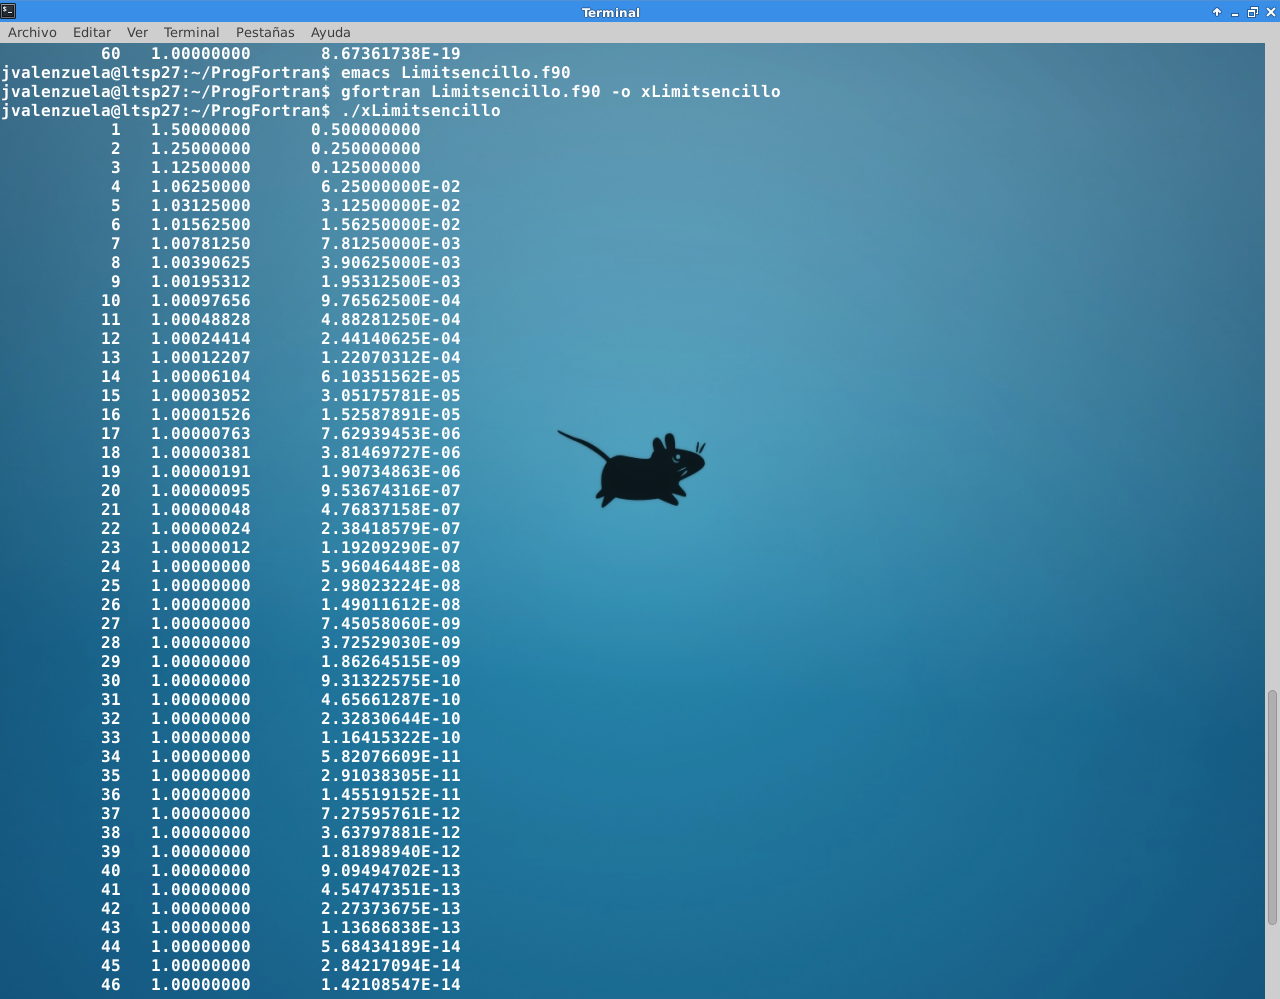
\includegraphics[scale=0.5]{Limitsencillo.png}

\end{figure}

\begin{verbatim}
!Limitsencillo.f90 Determines machine precision
Program Limitsencillo
  Implicit None
  Integer :: i , n
  Real *4 :: epsilon_m , one
  n=60 ! Establece el número de iteaciones
  ! Set initial values:
  epsilon_m = 1.0
  one = 1.0
  ! Within a DO-LOOP, calculate each step and print .
  ! This loop will execute 60 times in a row as i is
  ! incremented from 1 to n (since n = 60) :
  do i =  1, n , 1 ! Begin the do-loop
     epsilon_m = epsilon_m / 2.0 ! Reduce epsilon m
     one = 1.0 + epsilon_m ! Re-calculate one
     print *, i , one , epsilon_m ! Print values so far
     end do ! End loop when i>n
End Program Limitsencillo 
\end{verbatim}

\subsection{Funciones trigonométricas}

Fortran maneja funciones trigonométricas. Aquí un ejemplo de ello.

\begin{figure}[h]

\centering

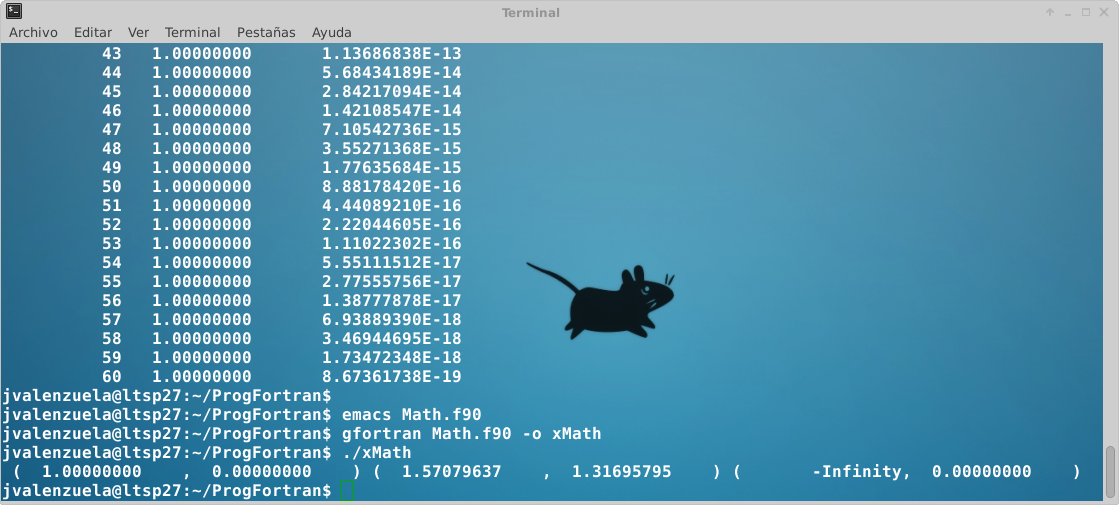
\includegraphics[scale=0.5]{Math.png}

\end{figure}

\begin{verbatim}
! Math.f90 : demostración de algunas funciones de fortran
Program Math  !Comienza el programa principal
  Complex *8 :: x= 1.0 , y=2 , z=0 !Declara las variabnles x, y , z
  x = sqrt (x) ! función razís cuadrada (square root)
  y= asin (y) ! Llama a la función arcoseno
  z= log (z) ! Función de exponencial
  print * , x, y, z ! Print x,y,z
End Program Math
\end{verbatim}

\subsection{Math modificado}

Se nos pide modificar el programa anterior para calcular la raíz cuadrada de -1, el arcoseno de 2 y el logaritmo de 0.

\begin{figure}[h]

\centering

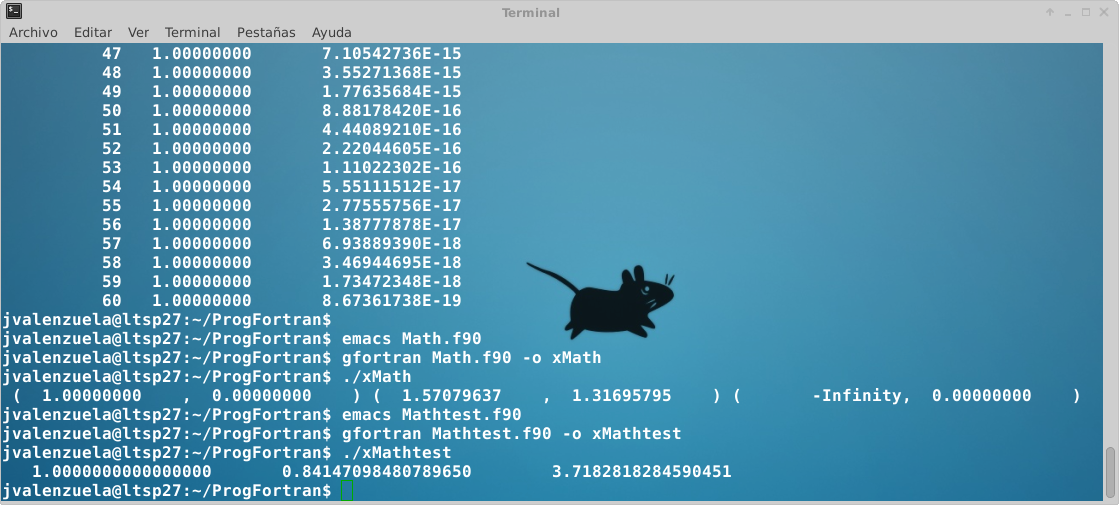
\includegraphics[scale=0.5]{Mathtest.png}

\end{figure}

\begin{verbatim}
Program Math_test
  real *8 :: x=1 , y, z
  y = sin (x)
  z = exp (x) + 1.00
  print * , x, y, z
  End Program Math_test
\end{verbatim}

\subsection{Función}

Se nos pide crear un programa que calcula el valor de una función f(x, y) = 1 + sin(x y) definida por el usuario

\begin{figure}[h]

\centering

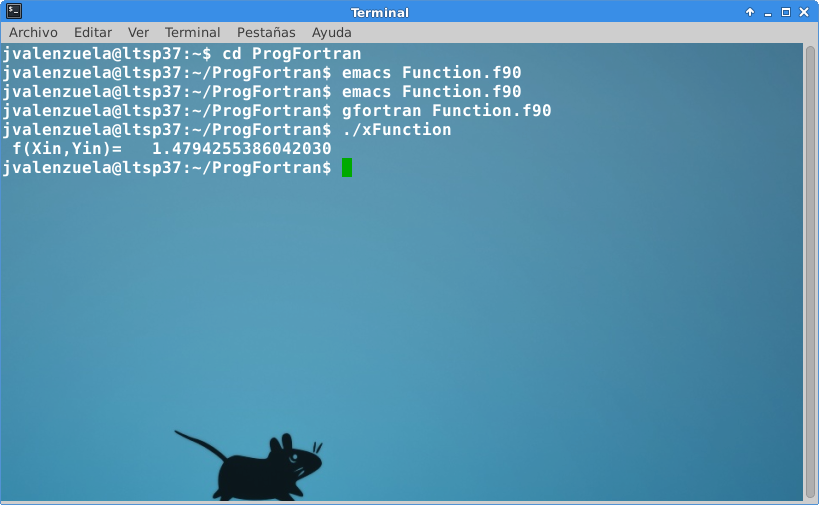
\includegraphics[scale=0.5]{Function.png}

\end{figure}

\begin{verbatim}
! Function . f90
Real *8 Function f (x,y)
  Implicit none
  Real *8 :: x, y
  f = 1.00 + sin (x*y)
  End Function f
!
  Program Main
    Implicit none
    Real*8 :: Xin =0.25, Yin =2.0, c, f !
    c= f ( Xin, Yin )
    write ( *,* ) 'f(Xin,Yin)=' , c
End Program Main
\end{verbatim}

\subsection{Subrutina}

Fortran además de funciones también maneja subrutinas. He aquí el ejemplo.

\begin{figure}[h]

\centering

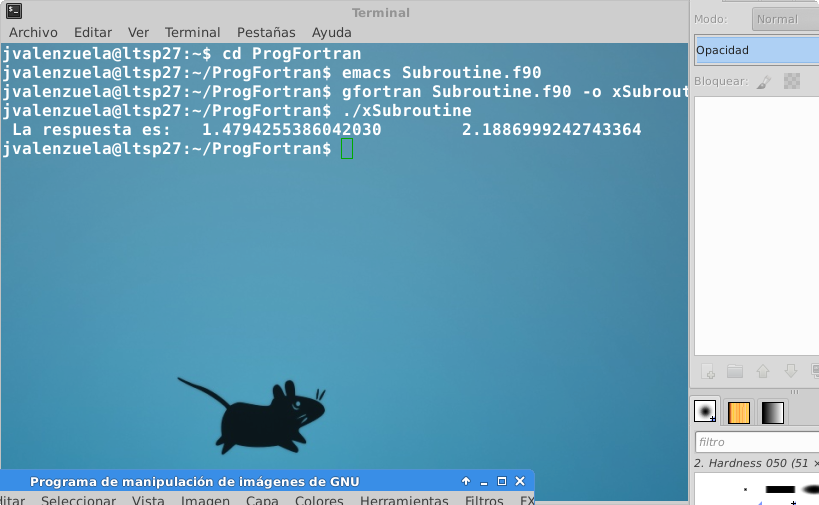
\includegraphics[scale=0.5]{Subroutine.png}

\end{figure}

\begin{verbatim}
  Subroutine g(x,y,ans1,ans2)
    Implicit None
    Real (8) :: x,y,ans1,ans2
    ans1 = sin (x*y) + 1
    ans2 = ans1**2
    End Subroutine g
!
Program Mainprogram
  Implicit None
  Real *8 :: Xin = 0.25, Yin = 2.00, Gout1, Gout2
  call g(Xin, Yin, Gout1, Gout2)
  write (*,*) 'La respuesta es:',Gout1, Gout2
End Program Mainprogram
\end{verbatim}

\end{document}
